\documentclass{beamer}
\usepackage[brazil]{babel}
%\usepackage[latin1]{inputenc}
\usepackage[utf8x]{inputenc} 
%\usepackage[all]{xy}

\usetheme{Antibes}

\title{Projeto de Tradução do GNOME para o Português do Brasil}

\author{Rodrigo L. M. Flores \\ \url{mail@rodrigoflores.org}}

\logo{
\includegraphics[width=1cm]{gnome-logo}}

\institute{GNOME Brasil}
\begin{document}

\date{\today}

\frame{\titlepage}

\section{Um pouco sobre nós}

\begin{frame}
    \frametitle{Missão}
    Fazer com que usuários do GNOME possam utilizar um sistema 
    totalmente traduzido para nosso idioma, cumprindo com padrões altos de qualidade 
\end{frame}

\begin{frame}
    \frametitle[Para o GNOME 2.28]{Nosso status}    
    \begin{itemize}[<+->]
        \item 100\% da Interface do Oficial 
        \item 87\% da Interface do Extra
        \item 82\% da Interface de Infraestrutura
        \item 36\% de Documentação do Oficial
        \item 9\%  de Documentação do Extra
        \item 31\% de Documentação de Infraestrutura
        \item Somos citados nas notas de lançamento desde o GNOME 2.4 (Setembro de 2003)  
    \end{itemize}

\end{frame}

\section{Como funcionavámos ?}

\begin{frame}
    \frametitle{Nosso fluxo de trabalho antigo}
    \begin{figure}[ht]
        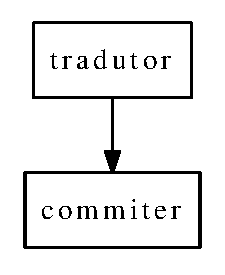
\includegraphics{fluxo_antigo.eps}     
    \end{figure}
\end{frame}

\begin{frame}
    \frametitle{Fluxo de tradução antigo}
    \begin{enumerate}[<+->]
        \item Tradutor escolhe um módulo não reservado no Wiki
        \item Tradutor baixa o arquivo po no Damned Lies
        \item Tradutor traduz o arquivo po
        \item Tradutor envia o arquivo po ao Bugzilla
        \item Um tradutor mais experiente revisa a tradução 
        \item Esse tradutor envia ao Bugzilla
        \item Commiter baixa a tradução do Bugzilla
        \item Commiter faz o commit no SVN
    \end{enumerate}
\end{frame}

\begin{frame}
    \frametitle{Falhas?}
    \begin{itemize}[<+->]
        \item Processo muito dependente do commiter
        \item Quase 30 módulos ficaram dependentes de revisão
        \item Reservas no Wiki as vezes eram esquecidas e aí módulos estavam ``pseudo-reservados''
        \item Processo muito complicado
    \end{itemize}

    Uma mudança então era necessária...
\end{frame}

\section{Uma nova era...}

\begin{frame}
    \frametitle{O que tinhamos?}
    \begin{itemize}[<+->]
        \item Além dos commiters (Leonardo Fontenelle e John Wendell), tinhamos tradutores com uma experiência boa (Vladimir Melo, Djavan Fagundes, entre outros);
        \item John Wendell sugeriu usarmos o Vertimus e começamos a utilizá-lo em produção;
    \end{itemize}
\end{frame}

\begin{frame}
    \frametitle{Nova proposta}  
    Em Abril de 2009, o Leonardo Fontenelle sugeriu uma nova proposta de organização da equipe:
    \begin{itemize}[<+->]
        \item Criação de uma nova classe: o revisor
        \item Promoção de um tradutor para revisor dependente principalmente dos outros revisores/committers
        \item Confiança no revisor
    \end{itemize}
\end{frame}

\begin{frame}
    \frametitle{Novo fluxo de trabalho}
    \begin{figure}[ht]
        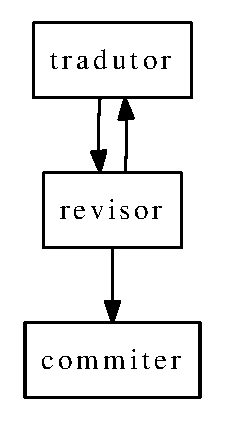
\includegraphics{fluxo_novo.eps}     
    \end{figure}
\end{frame}

\begin{frame}
    \frametitle[Vertimus]{Novo fluxo de tradução}
    \begin{itemize}[<+->]
        \item Tradutor reserva e baixa a tradução no Vertimus
        \item Tradutor sobe o arquivo traduzido ao Vertimus
        \item Revisor reserva a tradução
        \item Revisor sobe o arquivo revisado ao Vertimus
        \item Commiter baixa o arquivo do Vertimus
        \item Commiter avisa da submissão
    \end{itemize}
\end{frame}

\begin{frame}
    \frametitle{Resolve os falhas antigas ?}
    \begin{itemize}[<+->]
        \item Ainda somos dependentes dos Commiters, mas só para enviar tradução
        \item Traduções acumulam menos
        \item Reserva do módulo é redefinida a cada commit
        \item Processo bem mais simples
    \end{itemize}
\end{frame}

\begin{frame}
    \frametitle{E como tradutores viram revisores?}
    Através de um pedido na lista.

    Requisitos:
    \begin{itemize}[<+->]
        \item Fazer parte da equipe há, pelo menos, 6 meses
        \item Ter traduzido algum pacote ``não-trivial''
        \item Ser aprovado por pelo menos 2 commiters (e o coordenador pode ser um desses)
        \item Ser aprovado pelo coordenador
    \end{itemize}
\end{frame}

\begin{frame}
    \begin{block}{Contato}     
    \begin{itemize}
            \centering
            \item[E-mail] mail@rodrigoflores.org 
            \item[XMPP]  im@rodrigoflores.org        
            \item[Site]  \url{http://rodrigoflores.org}
            \item[Blog]  \url{http://blog.rodrigoflores.org}        
            \item[Twitter] rlmflores 
            \item[Identi.ca] rodrigoflores        
            \item[Jaiku] flores        
        \end{itemize}
    \end{block}
\end{frame}


\end{document}


% vim:set ts=4 expandtab:
